Find the explicit formula for the following wave equation
$$
\begin{cases}
  u_{tt} - \Delta u = 0, & x \in \reals^3, t > 0\\
  u(x, 0) = 0 & x \in \reals^3\\
  u_t(x, 0) = h(x) =
  \begin{cases}
    1 & |x| < 1\\
    0 & |x| > 1
  \end{cases} & x \in \reals^3
\end{cases}
$$
(Hint: $u$ is radially symmetric)

Just follow what we did in class :), trick to make it one dimensional.

Since $n = 3$, we can follow Kirchoff's formula.

Set

\begin{align*}
  U(x; r, t) = &\avgint_{\bndry{\ball{x}{r}}} u(y, t) \dd{S(y)}\\
  \tilde{U} = &r U\\
  H(x; r) = &\avgint_{\bndry{\ball{x}{r}}}
    \begin{cases}
      1 & |y| < 1\\
      0 & |y| > 1
    \end{cases}
    \dd{S(y)}\\
  \tilde{H} = &r H\\
\end{align*}

Note that $u(x, t) = \limitto{r}{0} U(x, r, t) = \limitto{r}{0} \frac{1}{r} \tilde{U}(x, r, t)$,
$h(x) = \limitto{r}{0} H(x, r) = \limitto{r}{0} \frac{1}{r} \tilde{H}(x, r)$.
Also note that $H(x; r)$ is the ratio of the spherical cap area in Figure \ref{spherecap} to the sphere's surface area.
\begin{figure}[ht]
  \begin{center}
    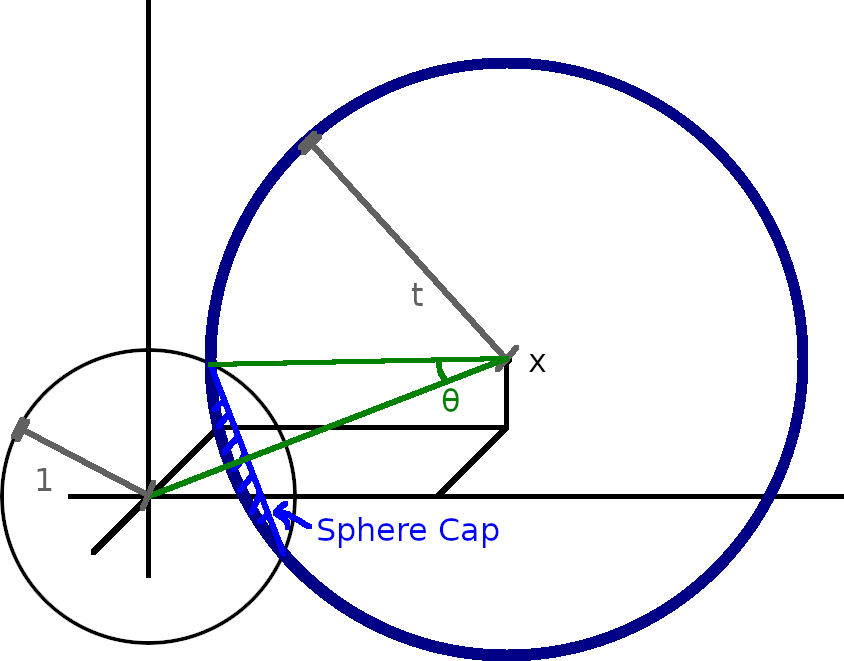
\includegraphics[width=0.5\textwidth]{spherecap.png}
  \end{center}
  \caption{Illustration of the sphere and sphere-cap the integral computes the area of}
  \label{spherecap}
\end{figure}

Then
\begin{align*}
  \tilde{U}_{tt} - \tilde{U}_{rr} = 0 & \text{ in } \reals_+ \times (0, \infty)\\
  \tilde{U} = \tilde{G}, \tilde{U}_t = \tilde{H} & \text{ on } \reals_+ \times \set{t = 0}\\
  \tilde{U} = 0 & \text{ on } \set{r = 0} \times (0, \infty)
\end{align*}

$$
u(x, t) = t \avgint_{\bndry{\ball{x}{t}}} h(y) \dd{S(y)}
$$

To compute the area of the spherical cap, we first note
$$
1 = t^2 \sin^2(\theta) + (|x| - t \cos(\theta))^2 = t^2 + |x|^2 - 2 |x| t \cos(\theta)
$$

Then, recall the surface area of a sphere cap for a sphere of radius $t$ and an angle $\theta$:
$$
A = 2 \pi t^2 (1 - \cos(\theta))
$$

Some manipulations of the previous two equations gives
$$
A = -\frac{\pi t}{|x|} \left( (|x| + t)^2 - 1 \right)
$$

Then, when $-1 < |x| - t < 1$ (since the sphere must actually intersect the unit sphere at the origin),
and $t \neq 0$, $u(x. t)$ is as follows:

$$
u(x, t) = t \frac{A}{4 \pi t^2} = -\frac{(|x| + t)^2 - 1}{4 |x|}
$$

In full:

$$
u(x, t) =
\begin{cases}
  -\frac{(|x| + t)^2 - 1}{4 |x|} & ||x| - t| < 1, t \neq 0\\
  0 & \text{otherwise}
\end{cases}
$$

To check our calculations, we can rewrite the original problem in spherical coordinates:

$$
\begin{cases}
  u_{tt} - \Delta u = u_{tt} - \frac{2}{r} u_r - u_{rr} = 0, & r > 0, \theta \in \reals^2, |\theta| = 1, t > 0\\
  u(r, \theta, 0) = 0 & r > 0, \theta \in \reals^2, |\theta| = 1\\
  u_t(r, \theta, 0) =
  \begin{cases}
    1 & r < 1\\
    0 & r > 1
  \end{cases} & r > 0, \theta \in \reals^2, |\theta| = 1
\end{cases}
$$

Our solution is

$$
u(r, \theta, t) =
\begin{cases}
  -\frac{(r + t)^2 - 1}{4 r} & |r - t| < 1, t \neq 0\\
  0 & \text{otherwise}
\end{cases}
$$

For $|r - t| < 1, t \neq 0$, we compute
\begin{align*}
  u_t = &\frac{t + r}{2 r}\\
  u_{tt} = &\frac{1}{2 r}\\
  u_r = &\frac{1 - t^2 + r^2}{4 r^2}\\
  u_{rr} = &\frac{t^2 - 1}{2 r^3}\\
  u_{tt} = &\frac{2}{r} u_r + u_{rr} = \frac{t^2 - 1}{2 r^3} - \frac{1}{2 r} + \frac{t^2 - 1}{2 r^3} = -\frac{1}{2 r}
\end{align*}

For $r < 1$, $\limitto{t}{0} u_t = \frac{1}{2}$, suggesting this is off by a factor of 2, so we amend the solution to
$$
u(r, \theta, t) =
\begin{cases}
  -\frac{(r + t)^2 - 1}{2 r} & |r - t| < 1, t \neq 0\\
  0 & \text{otherwise}
\end{cases}
$$
